\documentclass{article}[18pt]
\usepackage{/home/sam/Documents/School_Notes/format}
\lhead{AS Level Physics}

%File specific Preable
%Format paragraphs correctly
\setcounter{secnumdepth}{4}
\titleformat{\paragraph}
{\normalfont\normalsize\bfseries}{\theparagraph}{1em}{}
\titlespacing*{\paragraph}
{0pt}{3.25ex plus 1ex minus .2ex}{1.5ex plus .2ex}

\begin{document}
\begin{center}
\underline{\huge AS Physics}
\end{center}
\section{Matter and radiation}
\subsection{Inside the atom}
\subsubsection{Specific charge}
$$\text{Specific Charge}=\dfrac{\text{Charge}}{\text{Mass}}$$
\subsection{Stable and unstable nuclei}
\subsubsection{The strong force}
0fm - 0.5fm - Repulsion\\
0.5fm - 3fm - Attraction\\
3fm+ - No force\\
\subsubsection{Radioactive decay}
\paragraph{Alpha Radiation}
$$\mathsmaller{^A_Z}X\rightarrow\mathsmaller{^{A-4}_{Z-2}}Y+\mathsmaller{^4_2}\alpha$$
\paragraph{Beta radiation}
$$\mathsmaller{^A_Z}X\rightarrow\mathsmaller{^{A}_{Z+1}}Y+\mathsmaller{^0_{-1}}\beta+\overline{\nu}$$
\paragraph{Gamma Radiation}
This is emitted by an unstable nucleus. It has no mass and no charge. It is caused by a nucleus having too much energy, following an alpha or beta emissions.
\subsection{Photons}
\subsubsection{Electromagnetic waves}
$$\text{The power of a laser beam}=nhf$$
n is the number of photons that pass a fixed point in a second
\subsection{Particles and antiparticles}
\subsubsection{Antimatter}
\paragraph{$\mathbf{\beta^+}$ decay}
$$\mathsmaller{^A_Z}X\rightarrow\mathsmaller{^{A}_{Z-1}}Y+\mathsmaller{^0_{+1}}\beta+\nu$$
\paragraph{Theory of antiparticles}
For every type of particle, there is a corresponding antiparticle that:
\begin{itemize}
\item Annihilates the particle and itself if they meet, converting their total mass into photons
\item Has exactly the same rest mass as the particle
\item Has exactly opposite charge to the particle if the particle has a charge
\end{itemize}
\textbf{Pair production} - A photon with sufficient energy can change into a particle-antiparticle pair\\
\\
To find the energy of an electron, use $E=mc^2$
\subsection{How particles interact}
\subsubsection{The weak nuclear force}
This affects both leptons and quarks\\
\paragraph{Exchange particle}
The W bosons:
\begin{itemize}
\item Have a non-zero rest pass
\item Have a very short range (0.001fm)
\item Are positively charged($W+$) or negatively charged ($W^-$)
\end{itemize}
Strangeness is not conserved with the weak nuclear force
\subsection{Electron capture}
$$p+e^-\rightarrow n+\nu$$
\section{Quarks and leptons}
\begin{tabularx}{\textwidth}{|X|X|X|X|}
\hline
Particle&Charge&Antiparticle&Interaction\\
\hline
Proton&+1&Antiproton $\overline{p}$&Strong, weak, electromagnetic\\
\hline
Neutron&0&Antineutron $\overline{n}$&Strong, weak\\
\hline
Electron $e^-$&-1&Positron $e^+$&Weak, electromagnetic\\
\hline
Neutrino $\nu$&0&Antineutrino $\overline{v}$&Weak\\
\hline
Muon $\mu^-$&-1&Antimuon $\mu^+$&Weak, electromagnetic\\
\hline
$\pi$ meson $\pi^+,\pi^0,\pi^-$&+1,0,-1&Inverse symbol, $\pi^0$ is own antiparticle&Strong, electromagnetic (charged only)\\
\hline
K meson $K^+,K^0,K^-$&+1,0,-1&&Strong, electromagnetic (charged)\\
\hline
\end{tabularx}
\subsection{Leptons at work}
\subsubsection{Lepton rules}
\paragraph{Rule 1}
In an interaction between a \textbf{lepton} and a \textbf{hadron}, a neutrino or antineutrino can change into or from a corresponding charged lepton.
$$\nu_e+n\rightarrow p+e^-$$
\paragraph{Rule 2}
In \textbf{muon} decay, the muon changes into a muon neutrino. In addition an electron and electron neutrino are created to conserve charge.
$$\mu^-\rightarrow E^-+\overline{\nu_e}+\nu_\mu$$
\section{Quantum phenomena}
\subsection{Photoelectricity}
\subsubsection{The discovery of photoelectricity}
Observations made about photoelectricity:
\begin{enumerate}
\item Photoelectric emission of electron does take place if the frequency is below the \textbf{threshold} frequency
\item The number of electrons emitted per second is proportional to the intensity of the incident radiation
\item Photoelectric emission occurs instantaneously 
\end{enumerate}
\subsubsection{Formulae}
$hf=\phi+E_{Kmax}$\\
$\phi$ = $hf_0$ = Work Function - The minimum energy needed for an electron to escape from the metal surface\\
\subsection{Collisions of electrons with atoms}
\subsubsection{Ionisation}
\textbf{Ion} - An atom where the number of protons is not the same as the number of electrons\\
\textbf{Ionisation energy of a gas atom = eV}
\subsubsection{Excitation}
Excitation is where gas atoms absorb energy from electron collisions without ionising. This causes electrons to increase in the energy levels.
\subsection{Energy levels}
\subsubsection{Electrons in atoms}
\textbf{Ground state} - The lowest energy state of an atom\\
\textbf{Excited state} - An energy state above the ground state
\subsubsection{De-excitation}
Excited atoms are unstable and so will tend towards their ground state. When an electron moves down an energy level a photon is emitted with energy equivalent to the loss of energy by the electron.
\subsubsection{Excitation using photons}
An electron can absorb a photon and move to an outer shell where there is a vacancy. However the energy of the photon must be exactly the same as the gain of energy in the electron. If it is not then the photon will not be absorbed by the electron.
\subsection{Energy levels and spectra}
When the light from a filament lamp is split into a spectrum many discrete lines will be seen. These correspond to each of the energy levels of the atom
\subsection{Wave particle duality}
\textbf{Wave nature} - Diffraction\\
\textbf{Particle nature} - Photoelectric effect\\
\\
The wavelength of a matter particle is calculated by:
$$\lambda=\dfrac{h}{p}=\dfrac{h}{mv}$$\\
\section{Electric current}
\subsection{Potential difference and charge}
\textbf{Potential difference} - Work done per unit charge\\
\textbf{emf} - The electrical energy produced per unit charge passing through the source
\subsection{Resistance}
\subsubsection{Superconductivity}
A superconductor has \textbf{zero} resistivity at and below a \textbf{critical temperature}\\
Superconductors are used to make high-power electromagnets
\section{Direct current circuits}
\subsection{Circuit rules}
\subsubsection{Current}
\textbf{Series}: Current in = Current out. Current through multiple components is the same as through one\\
\textbf{Parallel}: Current into a junction = current out of a junction
\subsubsection{Voltage}
\textbf{Series}: Total voltage = the sum of voltages in the circuit\\
\textbf{Parallel}: Voltage in parallel components is equal
\subsection{Electromotive force and internal resistance}
\begin{tabularx}{\textwidth}{|X|X|}
\hline
Switch Open&Switch Closed\\
\hline
Voltmeter reads $\epsilon$&Voltmeter reads $\epsilon-IR$\\
\hline
\end{tabularx}
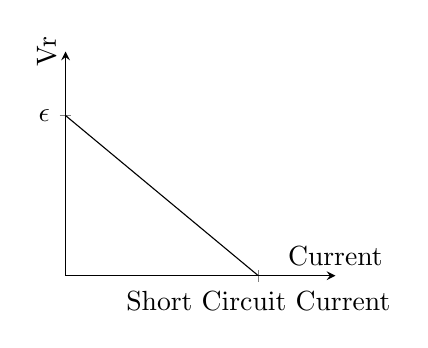
\begin{tikzpicture}
\begin{axis}[axis lines=middle,scale=0.5,    ylabel = Vr,xlabel=Current,ylabel style={rotate=90,anchor=south},xlabel style={anchor=south},xmin=0,xmax=7,ymin=0,ymax=7,xtick={5},xticklabels={Short Circuit Current},ytick={5},yticklabels={$\epsilon$}
]
\addplot[color=black,domain=0:5]{-x+5};
\end{axis}
\end{tikzpicture}
\subsection{The potential divider}
$$V_{Out}=V_{In}\times\dfrac{R_2}{R_1+R_2}$$\\
\\
Sensors reduce their resistance if the condition of the environment increases.
\section{Forces in equilibrium}
\subsection{Moments}
\subsubsection{Couples}
\textbf{Couple} - A pair of equal and opposite forces acting on a body\\
$$\text{Moment/Torque of a couple}=\text{Force}\times\text{Perpendicular distance between the lines of action of the forces}$$
\subsection{Stability}
\textbf{Stable} - Returns of equilibrium after displacement\\
\textbf{Unstable} - Does not return to equilibrium after displacement.
\subsubsection{Tilting and toppling}
An object will fall if the line of action of the centre of mass of the object lies outside the base.
\section{On the move}
\subsection{Speed and velocity}
\subsubsection{Speed}
\textbf{Displacement} - Distance in a given direction\\
\textbf{Speed} - Change of distance per unit time\\
\textbf{Velocity}- Change of displacement per unit time\\
\section{Motion and force}
\subsection{Newton's laws of motion}
\textbf{First law} - Objects either stay at rest or remain in uniform motion unless acted on by a force.\\
\textbf{Second law} - F=ma\\
\textbf{Third law} - Every action has an equal and opposite reaction\\
\\
\textbf{Inertia} - The resistance of an object to change its motion.
\subsubsection{Terminal speed}
The \textbf{drag force} depends on:Inertia
\begin{itemize}
\item The shape of the object
\item Its speed
\item The viscosity of the fluid the object is travelling through
\end{itemize}
\section{Waves}
\subsection{Waves and vibrations}
\subsubsection{Definitions}
\textbf{Displacement} - The distance and direction of a particle from its equilibrium position\\
\textbf{Amplitude} - The maximum displacement of a particle\\
\textbf{Wavelength} - The least distance between two adjacent vibrating particles with the same displacement and velocity at the same time\\
\textbf{One complete cycle} - From maximum displacement to the next maximum displacement\\
\textbf{Period} - The time for one complete wave to pass a fixed point\\
\textbf{Frequency} - The number of cycles of vibration of a particle per second.
\section{Optics}
\subsection{The diffraction grating}
\subsubsection{Types of spectra}
\paragraph{Continuous spectra}
The spectrum of light from a filament lamp is continuous. The hotter the light source, the shorter the wavelength of the brightest part of the spectrum.
\paragraph{Line emission spectra}
The light from a discharge tube emits light at specific wavelengths, meaning the spectra is of discrete lines. The wavelengths of the light are characteristic of the element that produces the light.
\paragraph{Line absorption spectra}
This is a continuous spectrum with narrow dark lines at certain wavelengths. This could be produced from the light from a filament lamp passing through a glowing gas. The elements in the gas absorb some of the photons, those that have exactly the correct energy to excite an electron.
\end{document}